\documentclass{article}
\usepackage{a4}
\usepackage{bm}
\usepackage{fullpage}
\usepackage{amsmath}
\usepackage{graphicx}
\usepackage{url}
\parindent 0pt
\parskip 6pt

\newcommand{\ku}{\mbox{\sf ku}}

\newcommand{\cb}{\bm{c}}
\newcommand{\kb}{\bm{k}}
\newcommand{\A}{\bm{A}}
\newcommand{\E}{\bm{E}}
\newcommand{\I}{\bm{I}}
\newcommand{\one}{\bm{1}} 
\newcommand{\vb}{\bm{v}} 
\newcommand{\tp}[1]{#1\!^{\top}}
\newcommand{\AT}{\tp{\A}}

\newcommand{\now}{\mbox{NOW}}
\begin{document}
This note is about cycles in the citation graph; their connection to
subsumption and possibly to web pages.

For an acyclic citation graph, I believe that we are all happy that
our standard model for credit transfer is reasonable.   The problem
happens when we introduce cycles where, even though the results for
kudos make sense and that we can show that what goes in must come out, we
can get large credit for nodes.  The simplest example is when we have
two documents $D_1$ and $D_2$.  $D_1$ sends all its credit to $D_2$
and  $D_2$ keeps 10\% of the kudos and transfers the remaining 90\% to
$D_1$.  Moreover, one unit of credit flows into $D_1$.

Following the notation in my ``notes'' document  ($\A$ is the
credit transfer matrix; $\cb$ $\vb$ and $\kb$ are vectors which give,
at each node, the credit, input and kudos; and $\one$ is a vector of
one)  we solve 
\[
\cb = \AT\cb+\vb\ \  \mbox{and}\ \   \kb = \cb -
(\A\one)\times\cb\ \  \mbox{when}\ \ 
\A = \left[\begin{array}{cc}
  0 & 1\\
  0.9 & 0
\end{array}\right]
\ \ and \ \ \vb = \left[\begin{array}{c} 0 \\ 1 \end{array}\right]
\]

which gives
\[ \kb = \left[\begin{array}{c} 0\\1 \end{array}\right] \ \ \ \ \cb =
\left[\begin{array}{c} 9\\10 \end{array}\right] \]

Why such a high credit total in each node?  In an acyclic graph the
credit at any node would surely be less than the total input to all
the ancestors of that node.

Maybe to explain this, consider the following acyclic structure
representing a simple, but highly artificial set of events.

\centerline{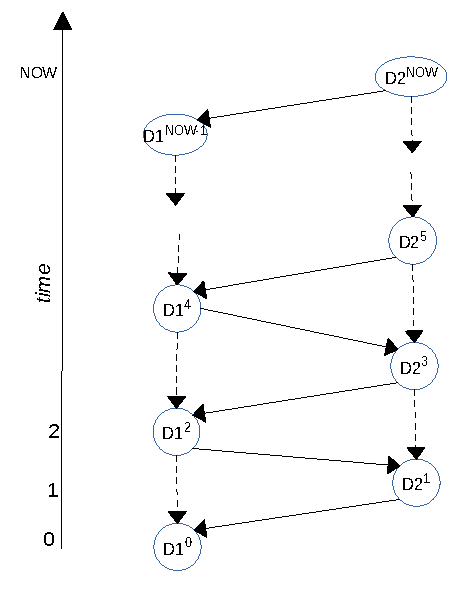
\includegraphics[scale=0.7]{zigzag.pdf}}

\begin{itemize}

\item
  At time 0, document $D_1^0$ is published. There's nothing to cite so
  it gets to keep all its input as kudos.

\item At time 1  $D_2^0$ is
published.  It  $D_1^0$ and transfers 90\% of its credit to
$D_1^0$. However $D_1^0$ does not necessarily receive credit for the
citation link 

\item At time 2, $D_1^2$  is published, which cites $D_2^1$. It decides to
transfer all its credit to $D_2^1$.  But again  $D_1^2$ does not
necessarily receive extra credit for the citation link from $D_2^1$

\item ... and so on, alternating until ...

\item Time $t^{\now}$, the present time.  In the picture, $\now$ is
    assumed to be odd.

\end{itemize}

Apart from having the same credit policy I have said nothing about the
relationship between $D_1^0, D_1^1, D_1^2\ldots$ and between $D_2^0,
D_2^1, D_2^2\ldots$.  Nor have I described the credit inputs.

Suppose just one credit is given to $D_2^{\now}$ then, with $\now = 8$,
we get 
\[
\begin{array}{rllll}
  t & D_1^t & D_2^t & k_1^t &k_2^t\\
  \hline
  8 & 0.0 & 1.0 & 0.0 & 0.1\\
7 & 0.9 & 0.0 & 0.0 & 0.0\\
6 & 0.0 & 0.9 & 0.0 & 0.09\\
5 & 0.81 & 0.0 & 0.0 & 0.0\\
4 & 0.0 & 0.81 & 0.0 & 0.081\\
3 & 0.729 & 0.0 & 0.0 & 0.0\\
2 & 0.0 & 0.729 & 0.0 & 0.0729\\
1 & 0.6561 & 0.0 & 0.0 & 0.0\\
0 & 0.0 & 0.6561 & 0.0 & 0.06561\\
\end{array}
\]

Not so interesting, but now suppose the vertical dotted arrows in the
figure above indicate 
(linear) subsumption; and suppose we $\now=100$.  I'm not going to show
the whole table, but since we have subsumption it make sense to add up
the kudos -- and the credit at each node.  That is, we add up the
columns to get:

\[ \kb = \left[\begin{array}{lc} 0\\0.995 \end{array}\right] \ \ \ \ \cb =
\left[\begin{array}{c} 8.95\\9.95 \end{array}\right] \]

Look familiar?   See above.  This is an explanation of why we see
large credit at nodes.

I'm not sure where this is going, but there are various questions.
First about subsumption. If A subsumes B:
\begin{itemize}
\item
If A (as is often the case)
cites B, should this add to the kudos of B -- and hence of A (the
subsuming document)?
\item If C cites both A and B does this count as one or two citations
  for A?
\item If both A and B cite C, does this count as one or two
    citations for B?
\end{itemize}
To make credit transfer work, I suspect that the answer to all three
questons has to be no.


More questions to follow, but an intriguing question is whether this
linear model of evolving subsumimg documents also serves as a model for web
pages.  If so there should be a connection with Page-rank.  Maybe it's
trivial.

\end{document}
